
%%%%%%%%%%%%%%%%%%%%%%%%%%%%%%%%%%%%%%%%%%%%%%%%%%%%%%%%%%%%%%%%%%%%%%%%%%%%%%%%%%%%%%%
%%%%%%%%%%%%%%%%%%%%%%%%%%%%%%%%%%%%%%%%%%%%%%%%%%%%%%%%%%%%%%%%%%%%%%%%%%%%%%%%%%%%%%%
%%%%%%%%%%%%%%%%%%%%%%%%%%%%%%%%%%%%%%%%%%%%%%%%%%%%%%%%%%%%%%%%%%%%%%%%%%%%%%%%%%%%%%%
\section{Derivadas notáveis: Gradiente, Matriz Hessiana, Matriz Jacobiana}

\index{Gradiente}
\begin{proposition}[$\triangledown e(\VECTOR{x})$ - Gradiente de $e(\VECTOR{x})$:]\label{def:gradient}
 Dada uma função $e:\mathbb{R}^{N}\rightarrow \mathbb{R}$ com variável $\VECTOR{x} \in \mathbb{R}^{N}$
 como vetor coluna com elementos $x_n\in \mathbb{R}$ de modo que $n\in \mathbb{N}$, $1 \leq n \leq N$,
 diferenciável em $\VECTOR{x}$. 
 $\triangledown e(\VECTOR{x})$ é chamado gradiente 
\cite[pp. 913]{stewart2008calculus} \cite[pp. 80]{telles2015matematica} \cite{Gradient}  de $e(\VECTOR{x})$, de modo que: 
\begin{equation}
\frac{\partial e(\VECTOR{x})}{\partial \VECTOR{x} }=
\left[
\begin{matrix}
\frac{\partial e(\VECTOR{x}) }{\partial x_{1}}&
\frac{\partial e(\VECTOR{x}) }{\partial x_{2}}&
\hdots&
\frac{\partial e(\VECTOR{x}) }{\partial x_{n}}&
\hdots&
\frac{\partial e(\VECTOR{x}) }{\partial x_{N}}
\end{matrix}
\right]^{\transpose}
 \end{equation}
\begin{equation}
\overrightarrow{\triangledown} e(\VECTOR{x})\equiv  
\triangledown e(\VECTOR{x}) \equiv 
\frac{\partial e(\VECTOR{x})}{\partial \VECTOR{x} }
\end{equation}
\end{proposition}


\noindent
\begin{minipage}{0.5\textwidth}
\begin{example}[Uso da Proposição \ref{def:gradient}:]
Conhecida a função $e(\VECTOR{x}): \mathbb{R}^2 \rightarrow \mathbb{R}$, 
\begin{equation}
e(\VECTOR{x})=x_1 e^{-x_1^2 - x_2^2},
\end{equation}
podemos calcular,
\begin{equation}
\frac{\partial e(\VECTOR{x}) }{\partial \VECTOR{x}}=
\begin{bmatrix}
(1-2 x_1^2) e^{-x_1^2 - x_2^2}\\
-2 x_1 x_2 e^{-x_1^2 - x_2^2}
\end{bmatrix}
\end{equation}
Um gráfico de $\frac{\partial e(\VECTOR{x}) }{\partial \VECTOR{x}}$ pode ser visto na Figura \ref{fig:ex:gradient}.
\end{example}
\end{minipage}
\begin{minipage}{0.45\textwidth}
    \begin{figure}[H]
	\centering
        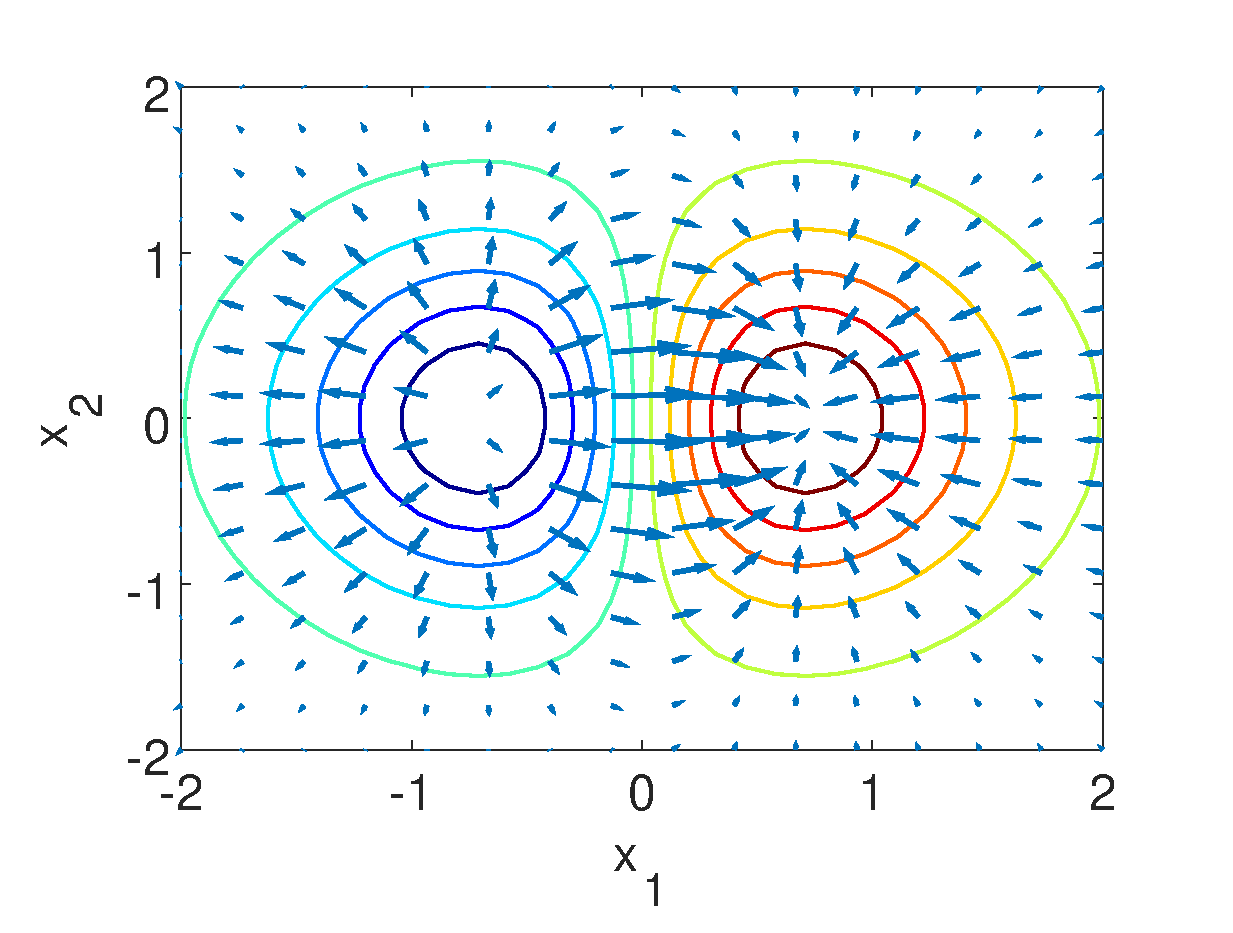
\includegraphics[width=\textwidth]{chapters/derivada/mfiles/gradiente/gradient.eps}
        \caption{Gráfico de $e(\VECTOR{x})$ como curvas de nível e $\triangledown e(\VECTOR{x})$ como vetores.}
        \label{fig:ex:gradient}
    \end{figure}
\end{minipage}

%%%%%%%%%%%%%%%%%%%%%%%%%%%%%%%%%%%%%%%%%%%%%%%%%%%%%%%%%%%%%%%%%%%%%%%%%%%%%%%%
\index{Matriz Jacobiana}
\begin{proposition}[Matriz Jacobiana de $\VECTOR{f}(\VECTOR{x})$:]\label{def:jacobian}
 Dado um vetor coluna, como função $\VECTOR{f}:\mathbb{R}^{N}\rightarrow \mathbb{R}^{M}$ com variável $\VECTOR{x} \in \mathbb{R}^{N}$
 como vetor coluna com elementos $x_n\in \mathbb{R}$ de modo que $n\in \mathbb{N}$, $1 \leq n \leq N$,
 diferenciável em $\VECTOR{x}$. 
 $\MATRIX{J}(\VECTOR{x})$ é chamada matriz Jacobiana \cite[pp. 130]{zhang2017matrix} \cite{Jacobian}  de 
 $\VECTOR{f}(\VECTOR{x})=[f_1(\VECTOR{x})~f_2(\VECTOR{x})~\dots~f_m(\VECTOR{x})~\dots f_M(\VECTOR{x})]^{\transpose}$, de modo que: 
 \begin{equation}
   \frac{\partial \VECTOR{f}(\VECTOR{x})}{\partial \VECTOR{x}^{\transpose} }=
\left[
\begin{matrix}
\frac{\partial \VECTOR{f}(\VECTOR{x}) }{\partial x_{1}}&
\frac{\partial \VECTOR{f}(\VECTOR{x}) }{\partial x_{2}}&
\hdots&
\frac{\partial \VECTOR{f}(\VECTOR{x}) }{\partial x_{n}}&
\hdots&
\frac{\partial \VECTOR{f}(\VECTOR{x}) }{\partial x_{N}}
\end{matrix}
\right]
 \end{equation}

\begin{equation}
\MATRIX{J}(\VECTOR{x})\equiv
\left[\overrightarrow{\triangledown} \VECTOR{f}^{\transpose}(\VECTOR{x})\right]^{\transpose} \equiv 
\frac{\partial \VECTOR{f}(\VECTOR{x})}{\partial \VECTOR{x}^{\transpose} }
\end{equation}

  \begin{equation}
  \MATRIX{J}(\VECTOR{x})\equiv 
\left[
\begin{matrix}
\frac{\partial f_1(\VECTOR{x}) }{\partial x_{1}}&
\frac{\partial f_1(\VECTOR{x}) }{\partial x_{2}}&
\hdots&
\frac{\partial f_1(\VECTOR{x}) }{\partial x_{n}}&
\hdots&
\frac{\partial f_1(\VECTOR{x}) }{\partial x_{N}}\\
\frac{\partial f_2(\VECTOR{x}) }{\partial x_{1}}&
\frac{\partial f_2(\VECTOR{x}) }{\partial x_{2}}&
\hdots&
\frac{\partial f_2(\VECTOR{x}) }{\partial x_{n}}&
\hdots&
\frac{\partial f_2(\VECTOR{x}) }{\partial x_{N}}\\
\vdots&
\vdots&
\hdots&
\vdots&
\vdots&
\vdots\\
\frac{\partial f_m(\VECTOR{x}) }{\partial x_{1}}&
\frac{\partial f_m(\VECTOR{x}) }{\partial x_{2}}&
\hdots&
\frac{\partial f_m(\VECTOR{x}) }{\partial x_{n}}&
\hdots&
\frac{\partial f_m(\VECTOR{x}) }{\partial x_{N}}\\
\vdots&
\vdots&
\hdots&
\vdots&
\vdots&
\vdots\\
\frac{\partial f_M(\VECTOR{x}) }{\partial x_{1}}&
\frac{\partial f_M(\VECTOR{x}) }{\partial x_{2}}&
\hdots&
\frac{\partial f_M(\VECTOR{x}) }{\partial x_{n}}&
\hdots&
\frac{\partial f_M(\VECTOR{x}) }{\partial x_{N}}\\
\end{matrix}
\right]
 \end{equation}
\end{proposition}


\begin{example}[Uso da Proposição \ref{def:jacobian}:]
Conhecida a função $\VECTOR{f}: \mathbb{R}^2 \rightarrow \mathbb{R}^2$,
onde $\VECTOR{u}=\VECTOR{f}(\VECTOR{x})$, 
\begin{equation}
\VECTOR{f}(\VECTOR{x})=
\begin{bmatrix}
\frac{x_1^3+x_2}{5}\\
\frac{x_2^3+x_1}{5}
\end{bmatrix}
\qquad \rightarrow \qquad
\frac{\partial \VECTOR{f}(\VECTOR{x}) }{\partial \VECTOR{x}^{\transpose}}\equiv
\MATRIX{J}(\VECTOR{x})\equiv
\begin{bmatrix}
\VECTOR{j}_{u_1}(\VECTOR{x})\\
\VECTOR{j}_{u_2}(\VECTOR{x})
\end{bmatrix}\equiv
\begin{bmatrix}
\frac{3 x_1^2}{5} & \frac{1}{5}\\
\frac{1}{5}       & \frac{3 x_2^2}{5}
\end{bmatrix}.
\end{equation}
Se $\VECTOR{\hat{x}}=[1~ 1]^{\transpose}$, usando a função $\VECTOR{f}(\VECTOR{\hat{x}})$ 
podemos calcular que $\VECTOR{\hat{u}}=[0.4~ 0.4]^{\transpose}$;
e usando a função $\MATRIX{J}(\VECTOR{\hat{x}})$ obtemos que $\VECTOR{j}_{u_1}(\VECTOR{\hat{x}})=[0.6~ 0.2]$ e $\VECTOR{j}_{u_2}(\VECTOR{\hat{x}})=[0.2~ 0.6]$.
Um gráfico do uso da matriz jacobiana avaliada em $\MATRIX{J}([1~ 1]^{\transpose})$ pode ser visto na Figura \ref{fig:ex:jacobiano}.
\end{example}

\begin{figure}[!h]
    \centering
    \begin{subfigure}[b]{0.49\textwidth}
        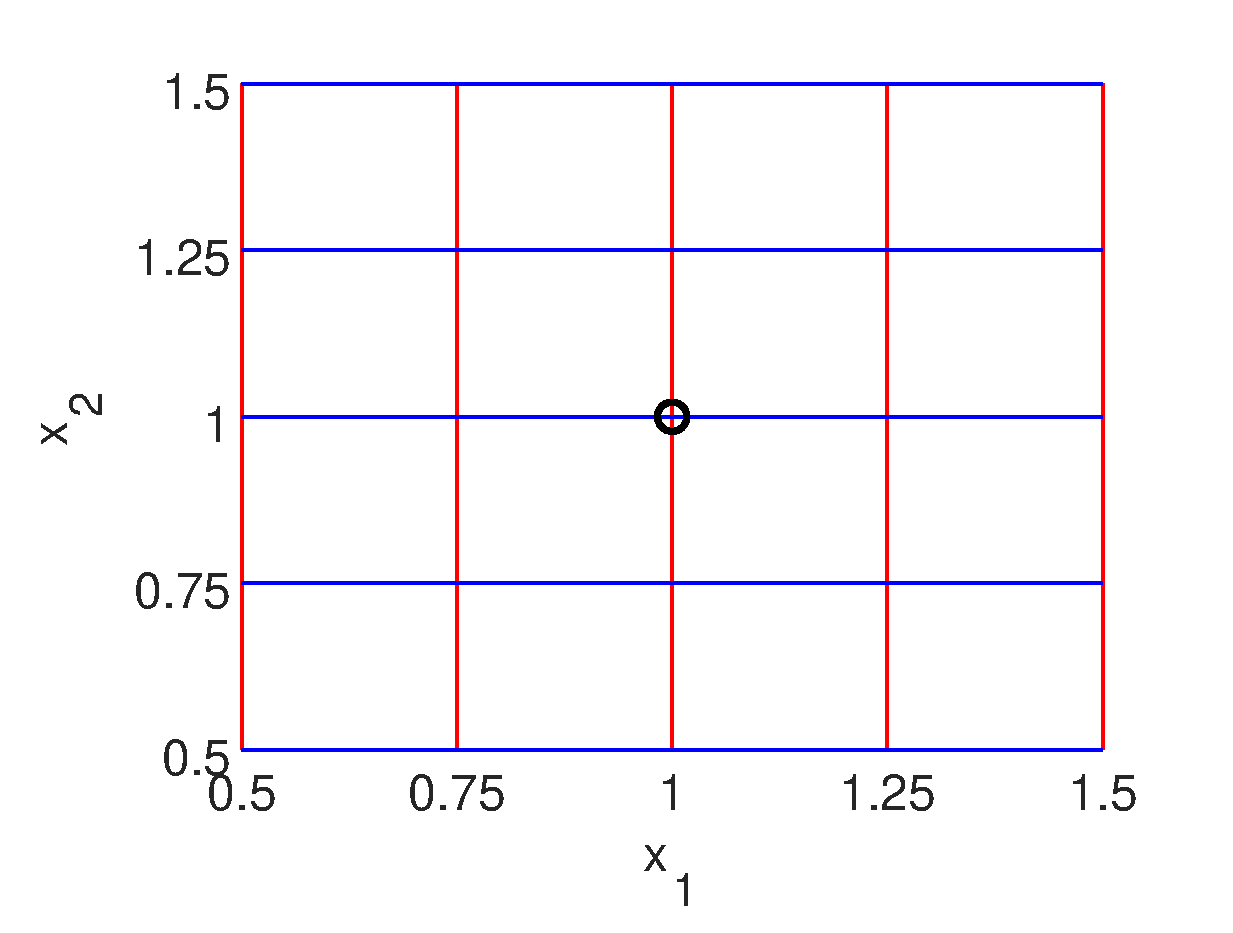
\includegraphics[width=\textwidth]{chapters/derivada/mfiles/jacobian/jacobian1.eps}
        \caption{Gráfico do ponto $\VECTOR{\hat{x}}$ e linhas auxiliares. ~~~~~~~~~ ~~~~~~~~~ ~~~~~~~~~}
        \label{fig:ex:jacobiano:x}
    \end{subfigure}
    ~ %add desired spacing between images, e. g. ~, \quad, \qquad, \hfill etc. 
      %(or a blank line to force the subfigure onto a new line)
    \begin{subfigure}[b]{0.49\textwidth}
        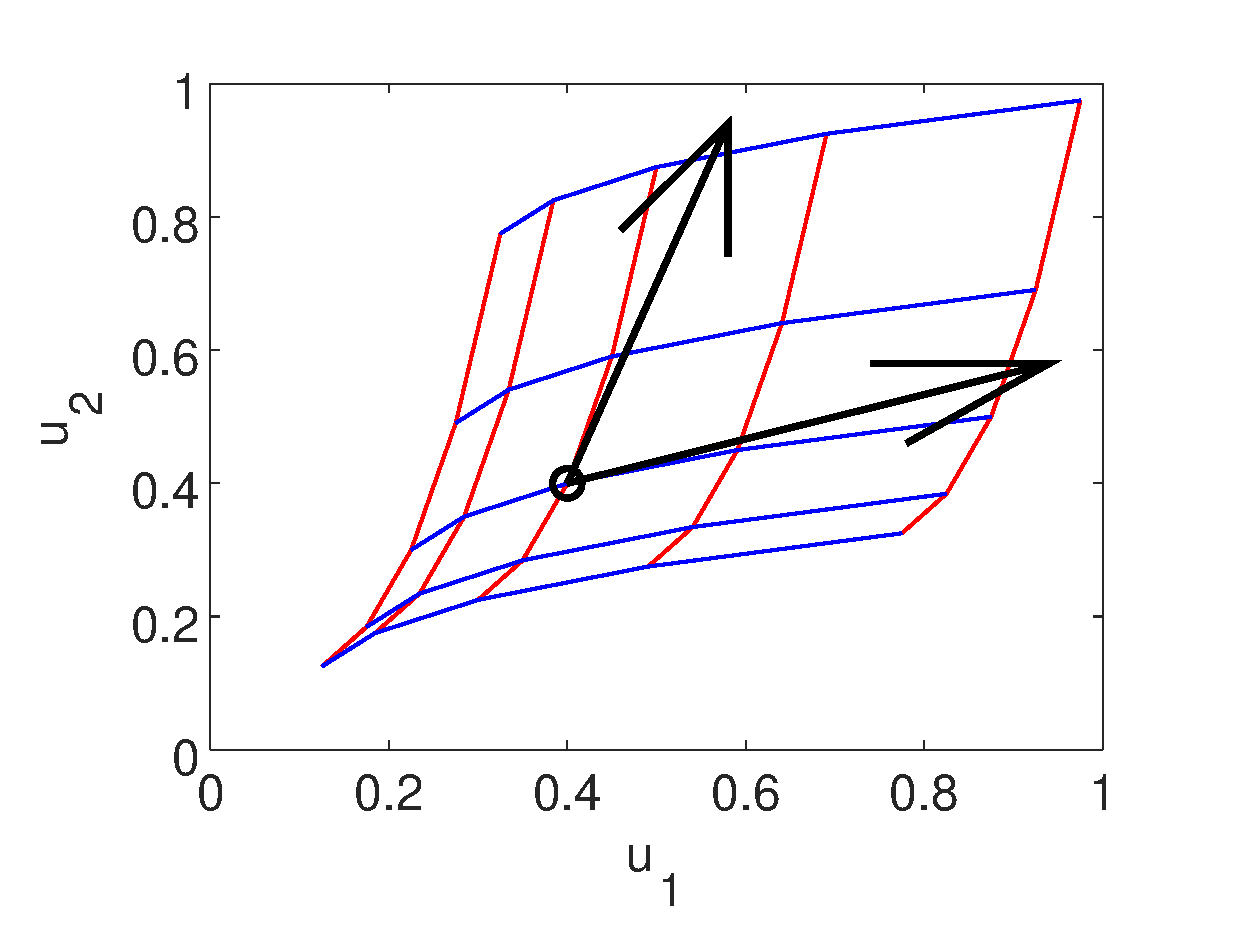
\includegraphics[width=\textwidth]{chapters/derivada/mfiles/jacobian/jacobian2.eps}
        \caption{Gráfico do ponto $\VECTOR{\hat{u}}$, dos vetores $\VECTOR{j}_{u_1}(\VECTOR{\hat{x}})$ e
    $\VECTOR{j}_{u_2}(\VECTOR{\hat{x}})$, e da avaliação das linhas auxiliares na função $\VECTOR{f}$.}
        \label{fig:ex:jacobiano:u}
    \end{subfigure}
    \caption{Gráfico do uso da matriz jacobiana.}
    \label{fig:ex:jacobiano}
\end{figure}


%%%%%%%%%%%%%%%%%%%%%%%%%%%%%%%%%%%%%%%%%%%%%%%%%%%%%%%%%%%%%%%%%%%%%%%%%%%%%%%%
\index{Matriz Hessiana}
\begin{proposition}[$\triangledown^2 e(\VECTOR{x})$ - Matriz Hessiana de $e(\VECTOR{x})$:]\label{def:hessian}
 Dada uma função $e:\mathbb{R}^{N}\rightarrow \mathbb{R}$ com variável $\VECTOR{x} \in \mathbb{R}^{N}$
 como vetor coluna  com elementos $x_n\in \mathbb{R}$ de modo que $n\in \mathbb{N}$, $1 \leq n \leq N$,
 diferenciável em $\VECTOR{x}$. 
 $\MATRIX{H}(\VECTOR{x})$ é chamada matriz Hessiana \cite[pp. 150]{zhang2017matrix} \cite{Hessian} 
 de $e(\VECTOR{x})$, de modo que: 
\begin{equation}
  \MATRIX{H}(\VECTOR{x}) \equiv  \overrightarrow{\triangledown} \overrightarrow{\triangledown}^{\transpose}e(\VECTOR{x}) \equiv  
\triangledown^2 e(\VECTOR{x}) \equiv \frac{\partial }{\partial \VECTOR{x}} \left( \frac{\partial e(\VECTOR{x})}{ \partial \VECTOR{x}^{\transpose} }\right) 
\end{equation}
 \begin{equation}
  \MATRIX{H}(\VECTOR{x}) =
\left[
\begin{matrix}
\frac{\partial^2 e(\VECTOR{x}) }{\partial x_{1}\partial x_{1}}&
\frac{\partial^2 e(\VECTOR{x}) }{\partial x_{1}\partial x_{2}}&
\hdots&
\frac{\partial^2 e(\VECTOR{x}) }{\partial x_{1}\partial x_{n}}&
\hdots&
\frac{\partial^2 e(\VECTOR{x}) }{\partial x_{1}\partial x_{N}}\\
\frac{\partial^2 e(\VECTOR{x}) }{\partial x_{2}\partial x_{1}}&
\frac{\partial^2 e(\VECTOR{x}) }{\partial x_{2}\partial x_{2}}&
\hdots&
\frac{\partial^2 e(\VECTOR{x}) }{\partial x_{2}\partial x_{n}}&
\hdots&
\frac{\partial^2 e(\VECTOR{x}) }{\partial x_{2}\partial x_{N}}\\
\vdots&
\vdots&
\vdots&
\vdots&
\vdots&
\vdots\\
\frac{\partial^2 e(\VECTOR{x}) }{\partial x_{m}\partial x_{1}}&
\frac{\partial^2 e(\VECTOR{x}) }{\partial x_{m}\partial x_{2}}&
\hdots&
\frac{\partial^2 e(\VECTOR{x}) }{\partial x_{m}\partial x_{n}}&
\hdots&
\frac{\partial^2 e(\VECTOR{x}) }{\partial x_{m}\partial x_{N}}\\
\vdots&
\vdots&
\vdots&
\vdots&
\vdots&
\vdots\\
\frac{\partial^2 e(\VECTOR{x}) }{\partial x_{M}\partial x_{1}}&
\frac{\partial^2 e(\VECTOR{x}) }{\partial x_{M}\partial x_{2}}&
\hdots&
\frac{\partial^2 e(\VECTOR{x}) }{\partial x_{M}\partial x_{n}}&
\hdots&
\frac{\partial^2 e(\VECTOR{x}) }{\partial x_{M}\partial x_{N}}\\
\end{matrix}
\right]
 \end{equation}
\end{proposition}



\index{Hesse, Ludwig Otto}
\begin{elaboracion}[title=Ludwig Otto Hesse (1811-1874), width= 0.99\linewidth]
Ele foi um matemático alemão que trabalhou em muitos temas como a matriz de Hessiana, 
o grupo Hessiano, os pares Hessianos, entre outras contribuições \cite[pp. 261]{agarwal2014creators}.
\end{elaboracion}
